% =====================================================================
% Project ESCAPE - Final Project Proposal (ACL-style submission version)
% Team Trimax - CS7.501 Advanced NLP
% Built on the real ACL style files (acl.sty / acl_natbib.bst).
% =====================================================================
\documentclass[9pt]{extarticle}
\usepackage[utf8]{inputenc}
\usepackage[T1]{fontenc}
\usepackage{acl}
% margin left at acl.sty's true default (2.5cm) -- no override
\usepackage{mathptmx} % Times, a standard academic serif -- denser than Computer Modern at the same point size
\usepackage{amsmath,amssymb}
\usepackage{url}
\usepackage{booktabs}
\usepackage{array}
\usepackage{enumitem}
\usepackage{tikz}
\usetikzlibrary{positioning}

% Tighter heading spacing than ACL's own \section/\subsection/\paragraph defaults
% (titlesec is unavailable on this TeX install, so redefine directly via \@startsection)
\makeatletter
\renewcommand\section{\@startsection{section}{1}{0pt}%
  {6pt plus 1pt minus 1pt}{4pt plus 1pt}{\normalfont\large\bfseries}}
\renewcommand\subsection{\@startsection{subsection}{2}{0pt}%
  {5pt plus 1pt minus 1pt}{3pt plus 1pt}{\normalfont\normalsize\bfseries}}
\renewcommand\paragraph{\@startsection{paragraph}{4}{0pt}%
  {5pt plus 1pt minus 1pt}{-1em}{\normalfont\normalsize\bfseries}}
\makeatother

\newcommand{\code}[1]{\texttt{\small #1}}
\setlist[itemize]{nosep,leftmargin=3.2mm,label=\textbullet}
\setlist[enumerate]{nosep,leftmargin=5mm}
\setlength{\intextsep}{6pt}
\setlength{\textfloatsep}{8pt}
\setlength{\floatsep}{6pt}
\renewcommand{\arraystretch}{0.92}

\title{\textbf{Project ESCAPE}: Entropy \& Semantic Compute Allocation in
Programming Environments: Structural Discovery via Entropy in the Byte Latent
Transformer Across Code and Natural Language \\[6pt]
{\normalsize\normalfont Team Trimax \quad$\cdot$\quad CS7.501 Advanced NLP \quad$\cdot$\quad Final Project Proposal}}

\author{
  Priyanka Agarwal\\ 2024101016
  \And Shashwat Mukadam\\ 2024102008
  \And Divyansh Atri\\ 2024113001
}

\begin{document}
\maketitle

\begin{abstract}
\noindent
Most language models split text using a fixed vocabulary learned before training,
such as byte-pair encoding. Every input is then chopped the same way, whether it
is boilerplate or dense logic. The Byte Latent Transformer (BLT)
\citep{pagnoni2024blt} does something different: it reads raw bytes and decides
where to split \emph{as it goes}, cutting whenever its own next-byte prediction
becomes uncertain. Those cut points are the model reporting where its knowledge
ran out.

Nobody has checked whether they mean anything. We ask a narrow, falsifiable
version of the question: \textbf{do BLT's boundaries land at the start of
syntactic constituents in code?} We call this the Grammatical Branching
Hypothesis. We give a mechanism for why it should hold, state plainly where that
mechanism must fail, and test it against a null model that holds boundary density
fixed, so a positive result cannot be dismissed as an artifact of BLT's
threshold $\tau$. Prose is a built-in negative control: if code and prose do not
separate, we are measuring $\tau$, not grammar. We further test whether an
entropy-only mechanism can be mistaken for semantic risk-awareness in
memory-unsafe C++, and test whether the two can be told apart. The protocol is
designed so that a null result is as informative as a positive one.
\end{abstract}

\section{Introduction}

Tokenization has been the standard front end for language models for a decade,
but it fixes a compression ratio in advance: a tokenizer trained before the
model sees your data spends the same number of tokens on boilerplate as on
subtle logic. BLT removes that fixed vocabulary. A small byte-level language
model, the \emph{patcher}, reads raw bytes and, at each position,
measures how uncertain it is about the next byte via Shannon entropy:
\begin{equation}
H(b_i) = -\sum_v p(v \mid b_{<i}) \log p(v \mid b_{<i})
\label{eq:entropy}
\end{equation}
When $H$ crosses a threshold $\tau$, BLT starts a new \emph{patch}, so a large
transformer spends more compute where bytes were hard to predict and less where
they were easy.

A boundary is therefore not a preprocessing decision but \textbf{a claim the
model makes about its own uncertainty}, interpretable in a way a BPE merge
table never is, since we can ask whether the claim corresponds to anything
independently verifiable. The BLT authors demonstrate the approach works, up to
8B parameters on 4T training bytes, but report only efficiency and downstream
accuracy; they never check whether the induced patches line up with structure we
can verify. That is the gap this project addresses, and code is the place to
look: it has machine-checkable ground truth in its abstract syntax tree (AST),
with grammar choice points that flexible prose does not have.

\section{Motivation and Related Work}

Interpretability work on tokenization has focused almost entirely on
\emph{static} vocabularies. Byte-pair encoding \citep{sennrich2016bpe} fixes a
merge table before training, with well-documented failure modes: poor
morphological alignment, unstable segmentation of rare or multilingual tokens.
Tokenization-free models remove the vocabulary but not the uniformity: CANINE
\citep{clark2022canine} and ByT5 \citep{xue2022byt5} process every byte with
equal compute, never deciding \emph{where} a boundary belongs, and BLT is the
first architecture at scale where segmentation is both byte-level and dynamic.

Structural probing work, including CodeBERT \citep{feng2020codebert} on code
and syntax probes on contextual representations \citep{hewitt2019structural},
shows \emph{learned representations} can encode syntax, but only because the
model was trained or probed \emph{for} that structure; none asks whether an
unsupervised, compression-only signal with no parser in the loop recovers
syntax as a side effect.

Two gaps follow: no work characterizes whether BLT's patcher implicitly
recovers constituent structure, and none establishes whether any such recovery
is genuine grammar-tracking or merely an artifact of patch density pinned by
$\tau$: a distinction that requires a principled null model, not a raw
overlap score.

\section{Contributions}

\begin{enumerate}
\item \textbf{A stated mechanism, not a black-box metric.} A specific, falsifiable
account (\S\ref{sec:why}) of \emph{why} boundaries should fall at constituent
starts, including explicit statement of where it must fail.
\item \textbf{A null model that makes the result mean something.} A
density-matched baseline plus a whitespace baseline (\S\ref{sec:pred}), so
measured alignment is attributable to grammar rather than to boundary density or
to newlines.
\item \textbf{A built-in negative control.} Prose is not a side experiment: the
same mechanism predicts a far weaker effect there, so failure to separate code
from prose is itself evidence we are measuring $\tau$.
\item \textbf{An honest scope limit.} We test what an entropy-only mechanism
\emph{cannot} see (\S\ref{sec:scope}), so we do not overclaim that surface
predictability implies danger-awareness.
\end{enumerate}

\section{Research Objectives}

\begin{enumerate}[label=\textbf{O\arabic*.}]
\item \textbf{Syntactic Alignment.} Do BLT's entropy-triggered boundaries align
with AST node boundaries in C++ and Python, beyond a density-matched baseline?
\item \textbf{Compute Allocation Ratio.} How do average Bytes-Per-Patch (BPP) and
its variance differ between rigid code syntax and natural language?
\item \textbf{Cross-Language Structural Recognition.} Does patching behave
differently for indentation-based syntax (Python) versus bracket-based (C++)?
\item \textbf{Robustness to Code Noise.} Do boundaries survive character-level
noise (syntax errors, obfuscation), or does the mechanism fail systemically?
\item \textbf{Semantic vs.\ Surface Compute Allocation.} Is any extra compute BLT
gives to memory-unsafe C++ operations \emph{fully explained} by the surface
unpredictability of nearby identifiers and casts, or does a residual remain after
conditioning on that confound?
\end{enumerate}

\section{Hypothesis}

\subsection{The Grammatical Branching Hypothesis (H1)}

BLT's patch boundaries are not random compression artifacts. They concentrate at
the \textbf{start} of syntactic constituents rather than inside them; this
concentration is stronger in code than in prose, and stronger at constituent
starts than at their ends.

Stated precisely, H1 claims an \emph{average-case asymmetry} between constituent
starts and constituent interiors. It does \textbf{not} claim that constituent
starts are points of maximal grammatical choice. \S\ref{sec:why} explains why
that stronger claim is false and why it is not needed. The project measures how
large the asymmetry actually is.

\subsection{Why We Expect This to Hold}
\label{sec:why}

BLT's patcher is a small byte-level language model with a short (512-byte)
context window, emitting a boundary whenever next-byte entropy crosses $\tau$. A
boundary therefore marks exactly one thing: \textbf{a position where the
preceding context stops determining what comes next.} Everything below follows
from that sentence, and we are careful to claim no more than it supports.

\paragraph{Entropy bounds branching; it does not track it.}
It is tempting to say entropy measures the local branching factor $B$, the
number of grammatically valid continuations. It does not: entropy depends on
the \emph{shape} of the distribution, not the size of its support, and the only
guaranteed relation is $H \le \log B$. Ten valid continuations with one carrying
$99\%$ of the mass give $H = 0.08$ nats, well below $\tau = 1.34$; four
equiprobable continuations give $H = 1.39$ nats and cross it. Branching is
necessary for high entropy but nowhere near sufficient.

What survives is the bound in one direction. A boundary \emph{certifies} the
local distribution was genuinely flat: $H > \tau$ implies $B > e^{\tau} \approx
3.8$, so every entropy-triggered boundary sits where at least four
continuations were live: a \textbf{subset} of high-branching positions,
where the grammar has not yet concentrated its mass on one continuation. This
yields a prediction we state in advance: \textbf{precision against constituent
starts should exceed recall.}

\paragraph{The load-bearing claim is about interiors, not starts.}
Our argument does not require constituent starts to be maximal-choice points,
only that entropy be lower \emph{inside} a committed production than at its
boundary: a structural property of context-free grammars, not a statistical
hope. Once a production is entered, admissible continuations are constrained by
the production itself: mid-keyword and mid-identifier bytes are cheap, and
closing delimiters (\code{;}, \code{)}, \code{\}}) are among the most
predictable bytes in a file, since the grammar requires them once committed
rather than choosing them. This is the asymmetry P2 rests on: boundaries are
pushed \emph{away from} interiors and right edges, and constituent starts
inherit them by elimination, not by being choice-maximal.

\paragraph{Where this mechanism does not hold.}
Two dissociations follow directly, because they hit \emph{different} metrics.
First, some constituents open deterministically: in both C++ and Python,
\code{if}, \code{for} and \code{while} are followed by a forced token, and
\code{def} must be followed by a name. These starts have branching factor near
one, so the mechanism predicts BLT will miss them, costing \textbf{recall},
tested directly via P4. Second, high entropy also arises where no constituent
opens at all: partway through an identifier, inside a string literal or
comment. These are lexical choice points, not grammatical ones, costing
\textbf{precision}, the confound isolated in \S\ref{sec:scope}. The patcher
measures next-byte predictability, conflating grammatical branching with
lexical arbitrariness; nothing in the architecture separates them.

Table~\ref{tab:example} walks one line of C++ through all three cases.

\begin{table}[t]
\small\centering
\begin{tabular}{@{}llcl@{}}
\toprule
Position & Entropy & Split? & Case \\
\midrule
\code{i} of \code{if}      & high & yes & correct \\
\code{(} after \code{if}   & low  & no  & \emph{missed} start \\
\code{x} of \code{x > 0}   & high & yes & lexical, not syntactic \\
\code{)} \code{;} \code{\}} & low & no  & correct (supports P2) \\
\bottomrule
\end{tabular}
\caption{The mechanism applied to \code{if (x > 0) \{ total += 1; \}}. Row 1 is
the effect we predict. Row 2 costs recall (forced opener). Row 3 costs precision
(identifier entropy). Row 4 is why starts should beat ends.}
\label{tab:example}
\end{table}

\paragraph{Prose is the contrast case.}
Branching factor is flatter across a sentence (content words are hard
everywhere, function words easy everywhere, and no formal rule forces a clause
to end with a specific character), so prose should show more uniform patch
lengths and weaker structural anchoring. \textbf{This code/prose gap is what
makes the claim one about grammar rather than about $\tau$.}

\subsection{Predictions and Null Model}
\label{sec:pred}

\paragraph{P1: Alignment.} Boundary positions match AST node start offsets, within
a tolerance $k$ fixed \emph{a priori} per language on a held-out calibration
split, well above baseline, for statement- and expression-level nodes.

\paragraph{P2: Asymmetry.} Alignment at node starts is clearly higher than at node
ends. Closing delimiters are low-entropy, so BLT should systematically miss right
edges. Span-IoU therefore \emph{understates} the effect; boundary
precision/recall against start offsets, not IoU, is our primary metric.

\paragraph{P3: Cross-domain contrast.} BPP variance is high in code and low in
prose, and P1-style alignment in prose (against a constituency parse) is near
chance. Code and prose must dissociate.

\paragraph{P4: Stratification by opener.} Alignment is measurably weaker for
constituent types with deterministic openers (\code{if\_statement},
\code{for\_statement}) than for open-ended ones (\code{expression\_statement},
\code{return\_statement}, assignment right-hand sides). P4 follows directly from
\S\ref{sec:why} and is the sharpest test that the mechanism running is the one we
claim: a generic ``entropy correlates with structure'' story does not predict it.

\paragraph{Null model (H0).} Agreement between patch boundaries and AST node
starts is no better than a density-matched random boundary set: the same number
of boundaries, patch lengths drawn from BLT's own empirical patch-length
distribution and laid out in shuffled order, truncating the final sampled patch
so the boundary set exactly spans the file.

This baseline is required, not optional: mean patch length is roughly pinned by
$\tau$, so \emph{any} boundary set of the right density scores nonzero raw
alignment, and only the margin over H0 is informative. We assess it with a
permutation test (10{,}000 resamples), reporting effect size with confidence
intervals rather than a raw overlap number.

\paragraph{Second baseline: whitespace.} H0 is structure-blind by construction,
so it cannot rule out the most obvious confound in code: most AST node starts
sit immediately after a newline and indentation, so a trivial ``split at every
newline'' rule would score well on P1. H1 is only interesting if BLT beats
\emph{that}, not merely chance, which matters most in Python, where
indentation \emph{is} the grammar. Alignment is additionally computed
\emph{per AST depth}, since every byte sits inside several nested nodes and
``alignment'' is undefined until granularity is fixed.

\paragraph{What counts as a result.} H1 is supported if P1 clears both baselines
with non-overlapping confidence intervals, P2 holds in the predicted direction,
P3 shows code/prose dissociation, and P4's stratification appears. Any subset
failing is reported as such; \S\ref{sec:notobvious} explains why each failure mode
is itself interpretable.

\subsection{Why the Result Is Not Obvious in Advance}
\label{sec:notobvious}

If H1 holds, an unsupervised, entropy-driven compressor recovers syntactic
constituent boundaries with no parser in the loop and no code-specific
tokenizer. If H1 fails, \emph{how} it fails is itself the signal: uniformly
\textbf{high} boundary entropy would mean the patcher is undertrained on code
and allocates compute blind to grammar (fixable by retraining on code);
uniformly \textbf{low} entropy would mean code is so compressible that $\tau$
rarely fires, so boundaries are density-limited rather than structure-driven.
The sharpest way H1 could lose outright is identifier entropy dominating and
swamping the syntactic signal, the precision failure of \S\ref{sec:why},
addressed directly in \S\ref{sec:scope}. Because each failure mode is
diagnosable rather than a single pass/fail outcome, the experiment is
informative regardless of which way the result goes.

\subsection{Scope Limit: What Entropy Cannot See}
\label{sec:scope}

The patcher is a short-context, surface-statistics model with no representation of
pointer aliasing, ownership, or memory safety. Tokens like \code{new},
\code{delete}, \code{*} and \code{\&} are short, frequent and lexically
predictable, so the mechanism of \S\ref{sec:why} predicts \textbf{low} entropy at
them, not high.

Consequently \textbf{we do not expect BLT to allocate compute by semantic risk}.
That claim would directly contradict the mechanism our own hypothesis relies on.
Any extra compute observed in memory-unsafe regions should instead come from the
arbitrary identifiers and casts that tend to surround pointer operations.

Objective~5 tests this directly: we condition memory-specific compute profiling on
identifier-token entropy via regression, and predict that any apparent
memory-safety effect shrinks toward zero once that confound is controlled. This is
a confound-isolation test, not a search for semantic understanding. A null result
here is informative, not a failed experiment.

\begin{figure*}[t]
\centering
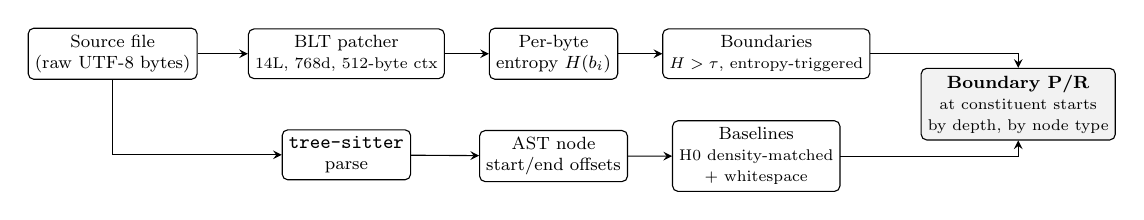
\begin{tikzpicture}[scale=0.80,transform shape,
  node distance=5mm,
  box/.style={draw,rounded corners=2pt,align=center,inner sep=3pt,font=\footnotesize,minimum height=7mm},
  lbl/.style={font=\scriptsize\itshape},
  >=stealth
]
\node[box] (src) {Source file\\(raw UTF-8 bytes)};
\node[box,right=8mm of src] (patch) {BLT patcher\\\scriptsize 14L, 768d, 512-byte ctx};
\node[box,right=7mm of patch] (ent) {Per-byte\\entropy $H(b_i)$};
\node[box,right=7mm of ent] (bnd) {Boundaries\\\scriptsize $H > \tau$, entropy-triggered};
\node[box,below=8mm of patch] (ts) {\code{tree-sitter}\\parse};
\node[box,below=8mm of ent] (ast) {AST node\\start/end offsets};
\node[box,right=7mm of ast] (base) {Baselines\\\scriptsize H0 density-matched\\\scriptsize + whitespace};
\node[box,right=8mm of bnd,yshift=-8mm,fill=black!5] (score)
  {\textbf{Boundary P/R}\\\scriptsize at constituent starts\\\scriptsize by depth, by node type};

\draw[->] (src) -- (patch);
\draw[->] (patch) -- (ent);
\draw[->] (ent) -- (bnd);
\draw[->] (src.south) |- (ts.west);
\draw[->] (ts) -- (ast);
\draw[->] (ast) -- (base);
\draw[->] (bnd.east) -| (score.north);
\draw[->] (base.east) -| (score.south);
\end{tikzpicture}
\caption{Extraction and scoring pipeline. The upper path is unsupervised: the
patcher never sees a parse tree. The lower path supplies independently verifiable
ground truth. Boundaries are scored against AST node starts and against both
baselines simultaneously, stratified by AST depth (\S\ref{sec:pred}) and by node
type (P4).}
\label{fig:pipeline}
\end{figure*}

\section{Methodology}
\label{sec:method}

Figure~\ref{fig:pipeline} shows the pipeline end to end.

\paragraph{Model and data.} We use \code{BltForCausalLM} from the Hugging Face
\code{transformers} library, specifically the \code{itazap/blt-1b-hf} checkpoint
(a 1B-parameter port of BLT's Local Encoder $\rightarrow$ Latent Transformer
$\rightarrow$ Local Decoder architecture, and the largest openly available BLT
checkpoint at present). Natural language is sampled from WikiText-103, Python
code from CodeSearchNet, and C++ from The Stack (\code{.cpp}/\code{.hpp} files;
CodeSearchNet has no C++ split). For the prose negative control (P3) we
additionally parse WikiText-103 sentences with a standard constituency parser
to obtain phrase-boundary ground truth.

\paragraph{Boundary extraction.} BLT resolves patches dynamically from the
entropy threshold ($\tau \approx 1.34$) and an optional maximum patch length;
the patcher exposes per-byte entropies and patch lengths directly, so
boundaries are read from its output rather than by instrumenting internals.
Each boundary is tagged \emph{entropy-triggered} or \emph{length-capped},
since a patch hitting the length cap before entropy crosses $\tau$ has nothing
to do with grammar, and length-capped boundaries are excluded from the
primary P1/P2 scores. Entropy is reported in nats, so $\tau = 1.34$ nats
$= 1.93$ bits.

\paragraph{Checkpoint fidelity.} The only public checkpoint is a third-party
conversion, so we sanity-check it before producing any numbers: coherent
generation, sensible boundaries on simple inputs, and, critically, that
the effective context window and patch-length distribution match those
reported in the original work, since the short window is load-bearing for
\S\ref{sec:why} and a silent mismatch would invalidate the mechanism we argue
from.

\paragraph{AST ground truth.} We parse code with \code{tree-sitter} for byte-level
start/end offsets of statement-level nodes (\code{if\_statement},
\code{for\_statement}, \code{declaration}) and expression-level nodes
(\code{call\_expression}, \code{binary\_expression}). Separately we query pointer
dereferencing (\code{*}), address referencing (\code{\&}) and manual memory
management (\code{new}/\code{delete}) as memory-unsafe regions.

\paragraph{Adversarial data.} We build a noised variant of the code corpus by
injecting missing semicolons, localized indentation changes,
camelCase$\leftrightarrow$snake\_case inversions, and typos in syntax keywords, to
probe robustness (O4). Noise breaks token patterns without destroying logical
validity; mutated files are re-parsed with \code{tree-sitter} and any that fail
to produce a clean tree are discarded, so degraded alignment cannot be blamed
on degraded ground truth.

\section{Evaluation Metrics}
\label{sec:metrics}

\begin{itemize}
\item \textbf{Boundary P/R at constituent starts (primary), overall and
stratified by node type.} Precision and recall of entropy-triggered boundaries
against AST node start offsets within tolerance $k$, as a margin over
\emph{both} baselines, and separately grouped by constituent type
(deterministic vs.\ open-ended openers, the test for P4). Where node types
share a start offset, a boundary is credited once, against the outermost
matching node, so nested starts cannot inflate precision. We expect
precision $>$ recall (\S\ref{sec:why}).
\item \textbf{AST boundary IoU (secondary).} Byte-span overlap between patches and
AST nodes; expected to understate the effect per P2, reported for comparability
with prior segmentation work.
\item \textbf{Compute density (BPP) and entropy heatmaps.} Bytes-per-patch
profiling and entropy visualizations over source text; we expect high BPP variance
for code versus more uniform BPP for prose.
\item \textbf{Degradation shift.} Change in the primary metric and in BPP between
clean and adversarial data, indicating robustness relative to subword tokenizers.
\item \textbf{Memory-specific compute profiling.} BPP in memory-unsafe regions
before and after conditioning on identifier-token entropy, isolating a genuine
semantic-risk effect (if any) from the surface-predictability confound.
\end{itemize}

\section{Feasibility and Compute}

The study is deliberately cheap: everything H1 requires comes from the
\emph{patcher} (roughly 150M parameters; see Figure~\ref{fig:pipeline}), never
the 1B latent transformer. Inference in \code{bfloat16} fits
on a single consumer GPU as a forward pass with no training, so the experiment
is reproducible on modest hardware; larger corpus sweeps and the adversarial
condition (O4) can dispatch as institutional batch jobs if throughput becomes
the limit. \textbf{No model training is required at any stage.}

\section{Risks and Mitigations}

\noindent
\begin{center}
\small
\begin{tabular}{@{}p{2.4cm}p{5.5cm}@{}}
\toprule
\textbf{Risk} & \textbf{Mitigation} \\
\midrule
Checkpoint infidelity &
Verified against the original configuration before any results are produced
(\S\ref{sec:method}); gates everything downstream. \\[1pt]
Newline confound &
Explicit whitespace baseline (\S\ref{sec:pred}); H1 must beat it, not merely H0. \\[1pt]
Identifier entropy swamps syntax &
Predicted in advance (\S\ref{sec:why}), isolated by regression in O5; recall
loss is total but confined to few node types, so precision should still net
dominate. \\[1pt]
Mechanism argued from bracket syntax &
Direct for C++'s closing delimiters; Python dedents instead, so O3, not
theory, decides whether interiors stay cheap there. \\[1pt]
Parser offset drift &
Character offsets round-tripped to UTF-8 byte offsets and validated before scoring. \\[1pt]
Depth incomparable across languages &
Alignment computed per depth and normalized before cross-language comparison (O3). \\
\bottomrule
\end{tabular}
\captionof{table}{Principal risks and how each is handled. The first is a
precondition, resolved in Weeks 1--3 before any alignment number is generated.}
\label{tab:risks}
\end{center}

\section{Deliverables}

The boundary-extraction pipeline (\S\ref{sec:method}), the \code{tree-sitter}
mapping engine, and the evaluation harness implementing P1--P4 and both
baselines (\S\ref{sec:metrics}) are each runnable independently. The
project's deliverable is a final report and presentation covering all five
objectives, including negative results.

\section{Timeline}

\begin{center}
\small
\begin{tabular}{@{}p{1.1cm}p{5.9cm}@{}}
\toprule
\textbf{Weeks} & \textbf{Work} \\
\midrule
1--3   & Extraction pipeline; \code{tree-sitter} AST mapping for Python/C++;
          checkpoint and context-window sanity checks. \\
4--6   & H0 null model and whitespace baseline; P1/P2 alignment on code; P4
          stratification; prose contrast (P3). \\
7--8   & Mid-submission write-up; adversarial dataset; O4. \\
9--11  & Memory-unsafe profiling and confound conditioning (O5); cross-language
          comparison (O3). \\
12+    & Consolidation, ablations, final write-up and presentation. \\
\bottomrule
\end{tabular}
\captionof{table}{Tentative timeline.}
\label{tab:timeline}
\end{center}

\begin{thebibliography}{9}
\footnotesize\setlength{\itemsep}{1pt}\setlength{\parskip}{0pt}
\bibitem[Clark et al.(2022)]{clark2022canine} Jonathan H. Clark, Dan Garrette,
Iulia Turc, and John Wieting. 2022. CANINE: Pre-training an efficient
tokenization-free encoder for language representation. \emph{TACL}, 10:73--91.
\bibitem[Feng et al.(2020)]{feng2020codebert} Zhangyin Feng et al. 2020.
CodeBERT: A pre-trained model for programming and natural languages.
\emph{Findings of EMNLP 2020}, pages 1536--1547.
\bibitem[Hewitt and Manning(2019)]{hewitt2019structural} John Hewitt and
Christopher D. Manning. 2019. A structural probe for finding syntax in word
representations. \emph{NAACL-HLT}, pages 4129--4138.
\bibitem[Pagnoni et al.(2024)]{pagnoni2024blt} Artidoro Pagnoni et al. 2024.
Byte Latent Transformer: Patches scale better than tokens. \emph{arXiv preprint
arXiv:2412.09871}.
\bibitem[Sennrich et al.(2016)]{sennrich2016bpe} Rico Sennrich, Barry Haddow, and
Alexandra Birch. 2016. Neural machine translation of rare words with subword
units. \emph{ACL}, pages 1715--1725.
\bibitem[Xue et al.(2022)]{xue2022byt5} Linting Xue et al. 2022. ByT5: Towards a
token-free future with pre-trained byte-to-byte models. \emph{TACL}, 10:291--306.
\end{thebibliography}

\end{document}
